\chapter{Multi view terrestrial laser scan registration}

\begin{figure}
	\centering
	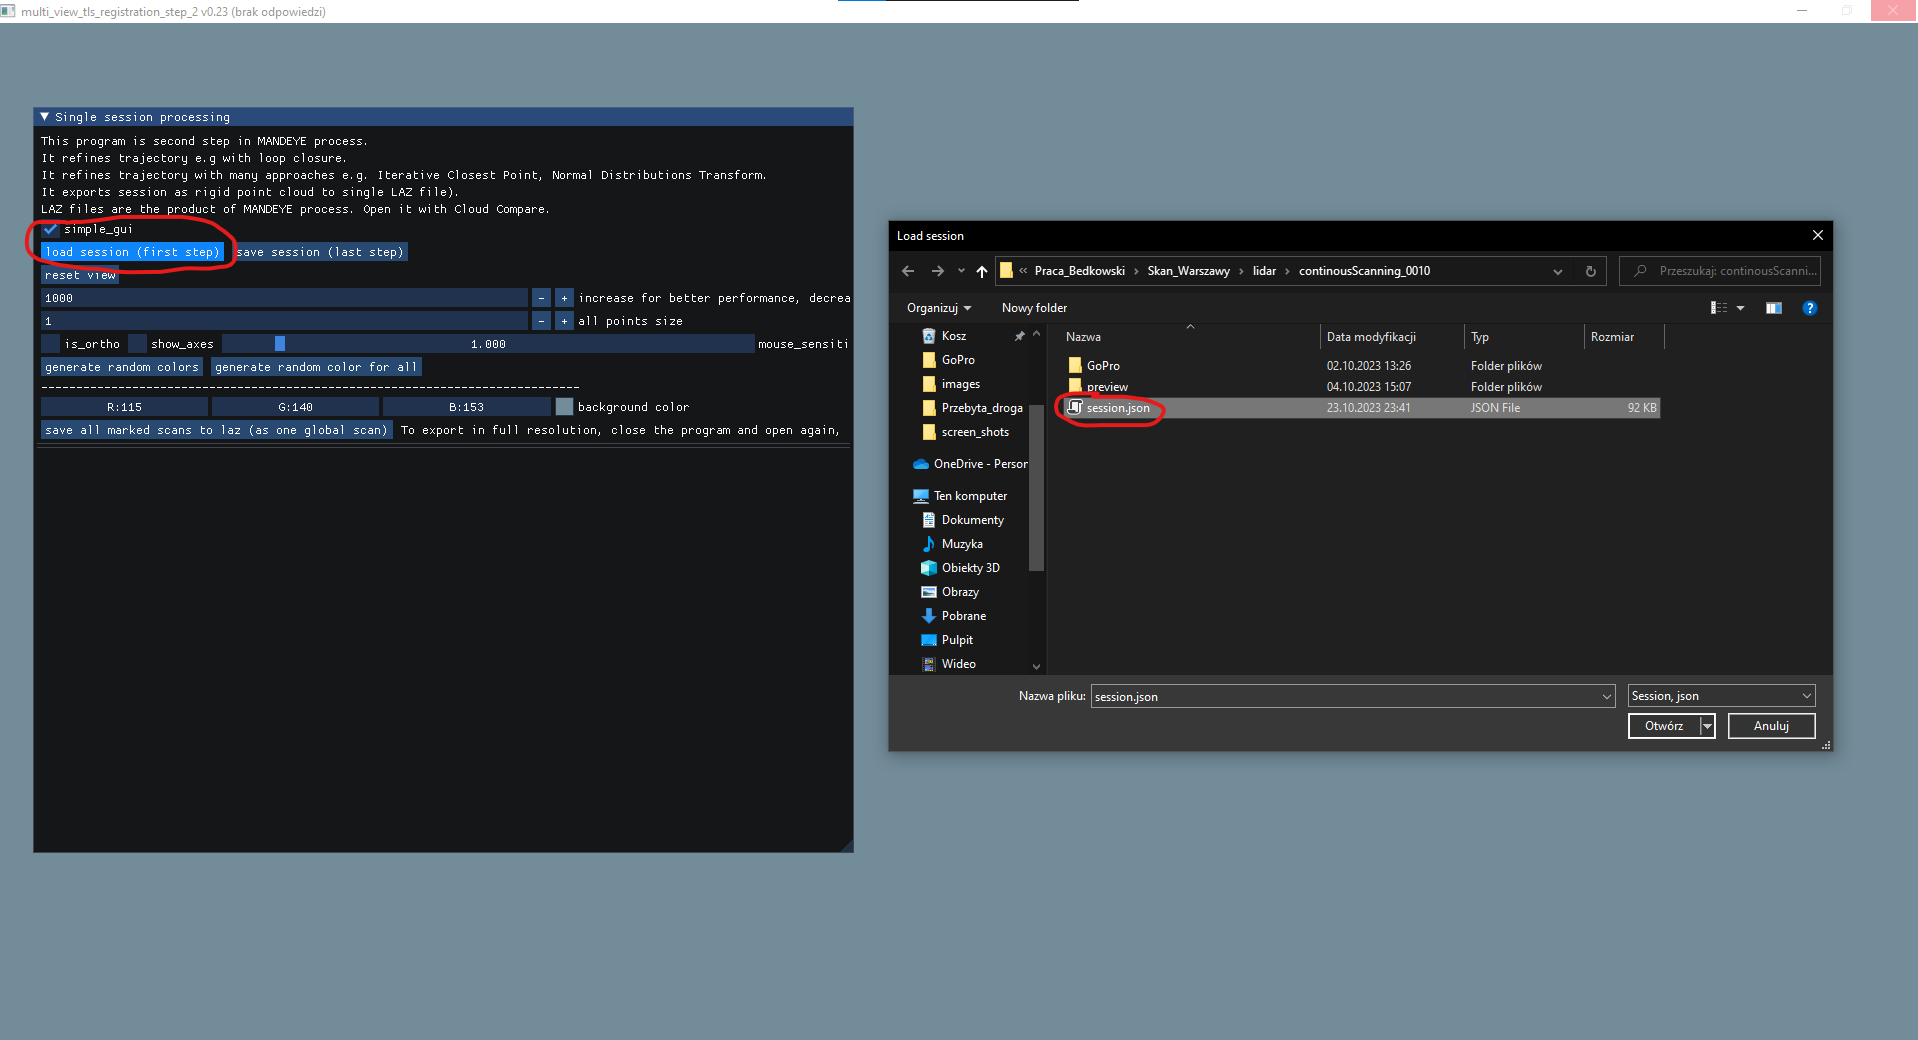
\includegraphics[width=\textwidth]{10.png}
	\caption{Load session.json prepared by 'Lidar odometry'.}
	\label{fig:10}
\end{figure}

\begin{figure}
	\centering
	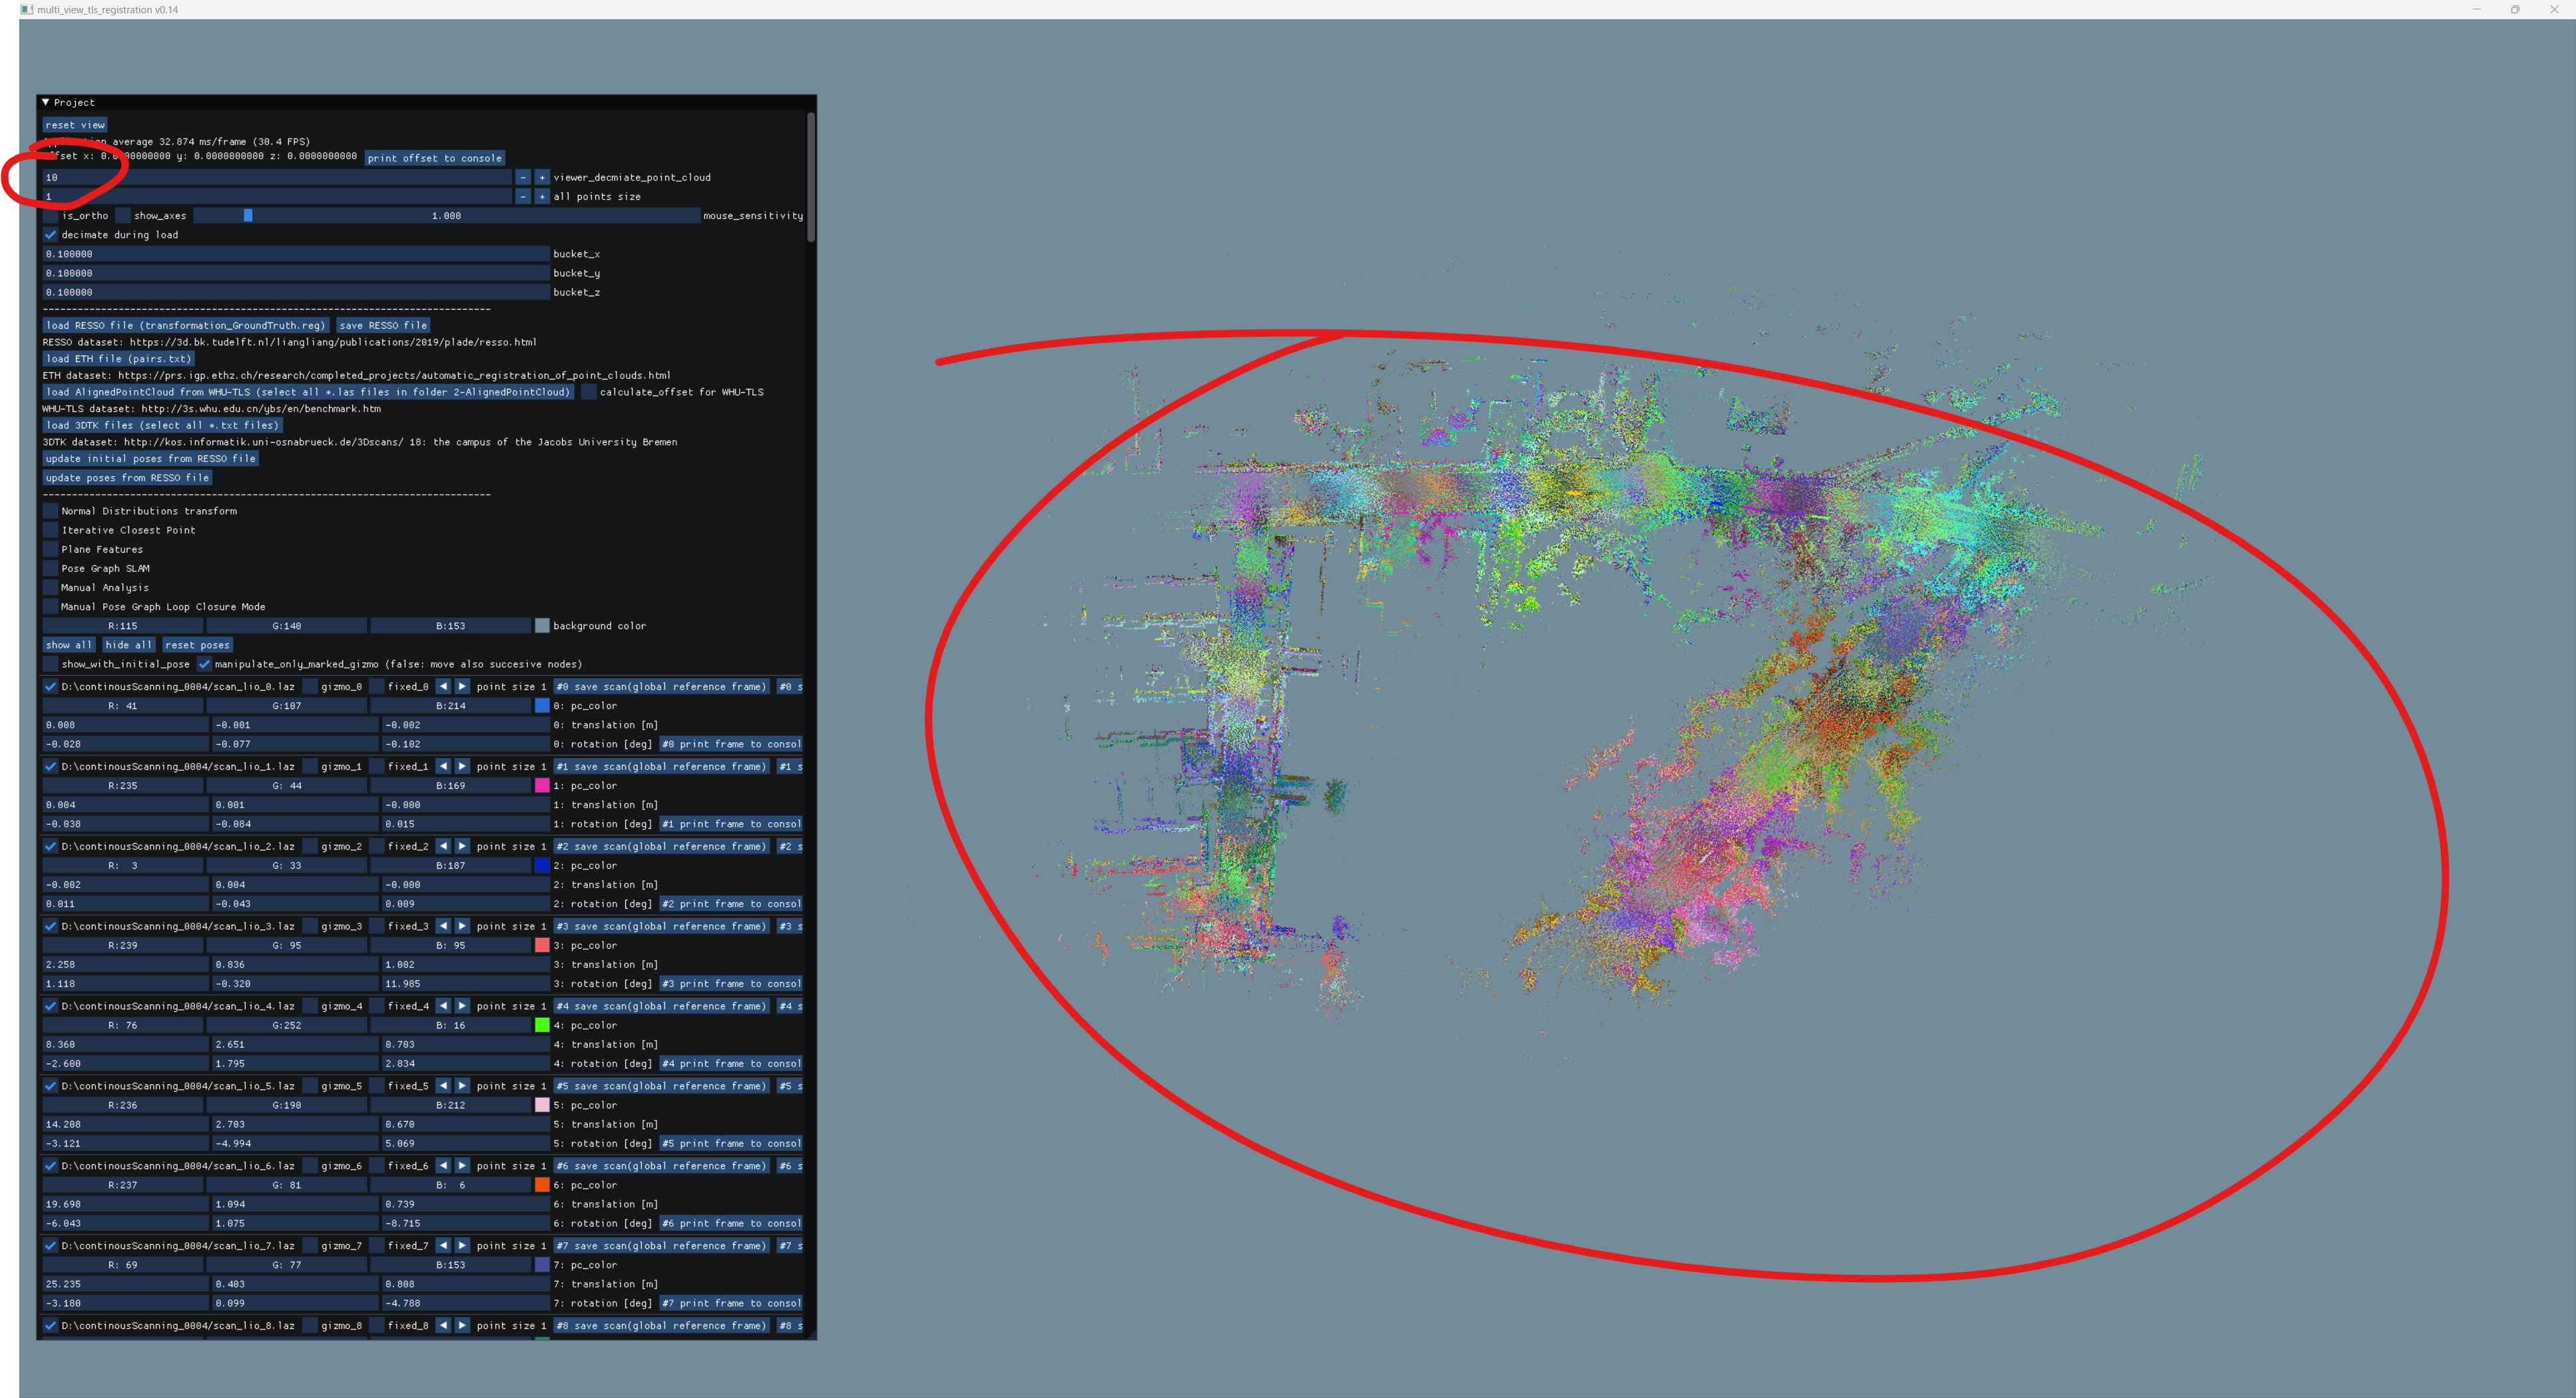
\includegraphics[width=\textwidth]{13.png}
	\caption{Prepare field of view and change decimation to see more points. Generate random colors option is recommended for next steps as every scan will be in a different color.}
	\label{fig:13}
\end{figure}

\begin{figure}
	\centering
	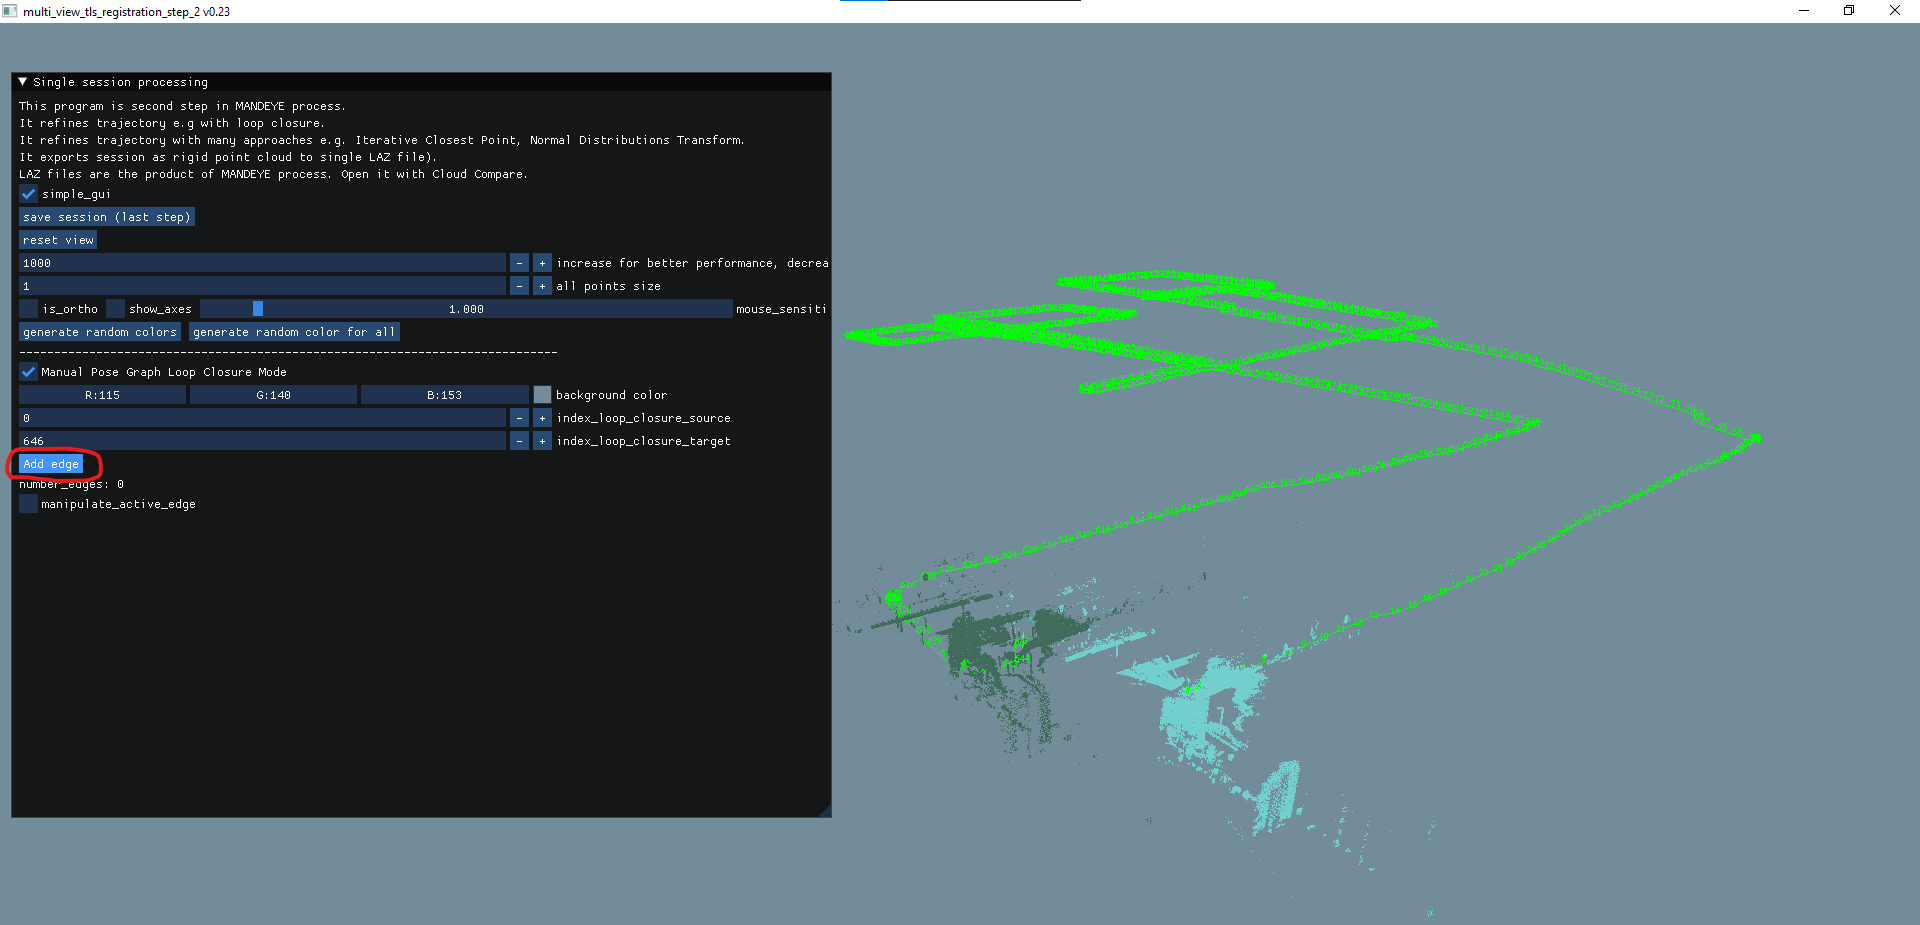
\includegraphics[width=\textwidth]{14.png}
	\caption{Turn on Manual Pose Graph Loop Closure Mod, then choose two different scans that share scanned objects, but difference in their numbers is as big as possible e.g. when you made a loop during scanning and came back to the same place after some time. Then click add edge.} 
	\label{fig:14}
\end{figure}

\begin{figure}
	\centering
	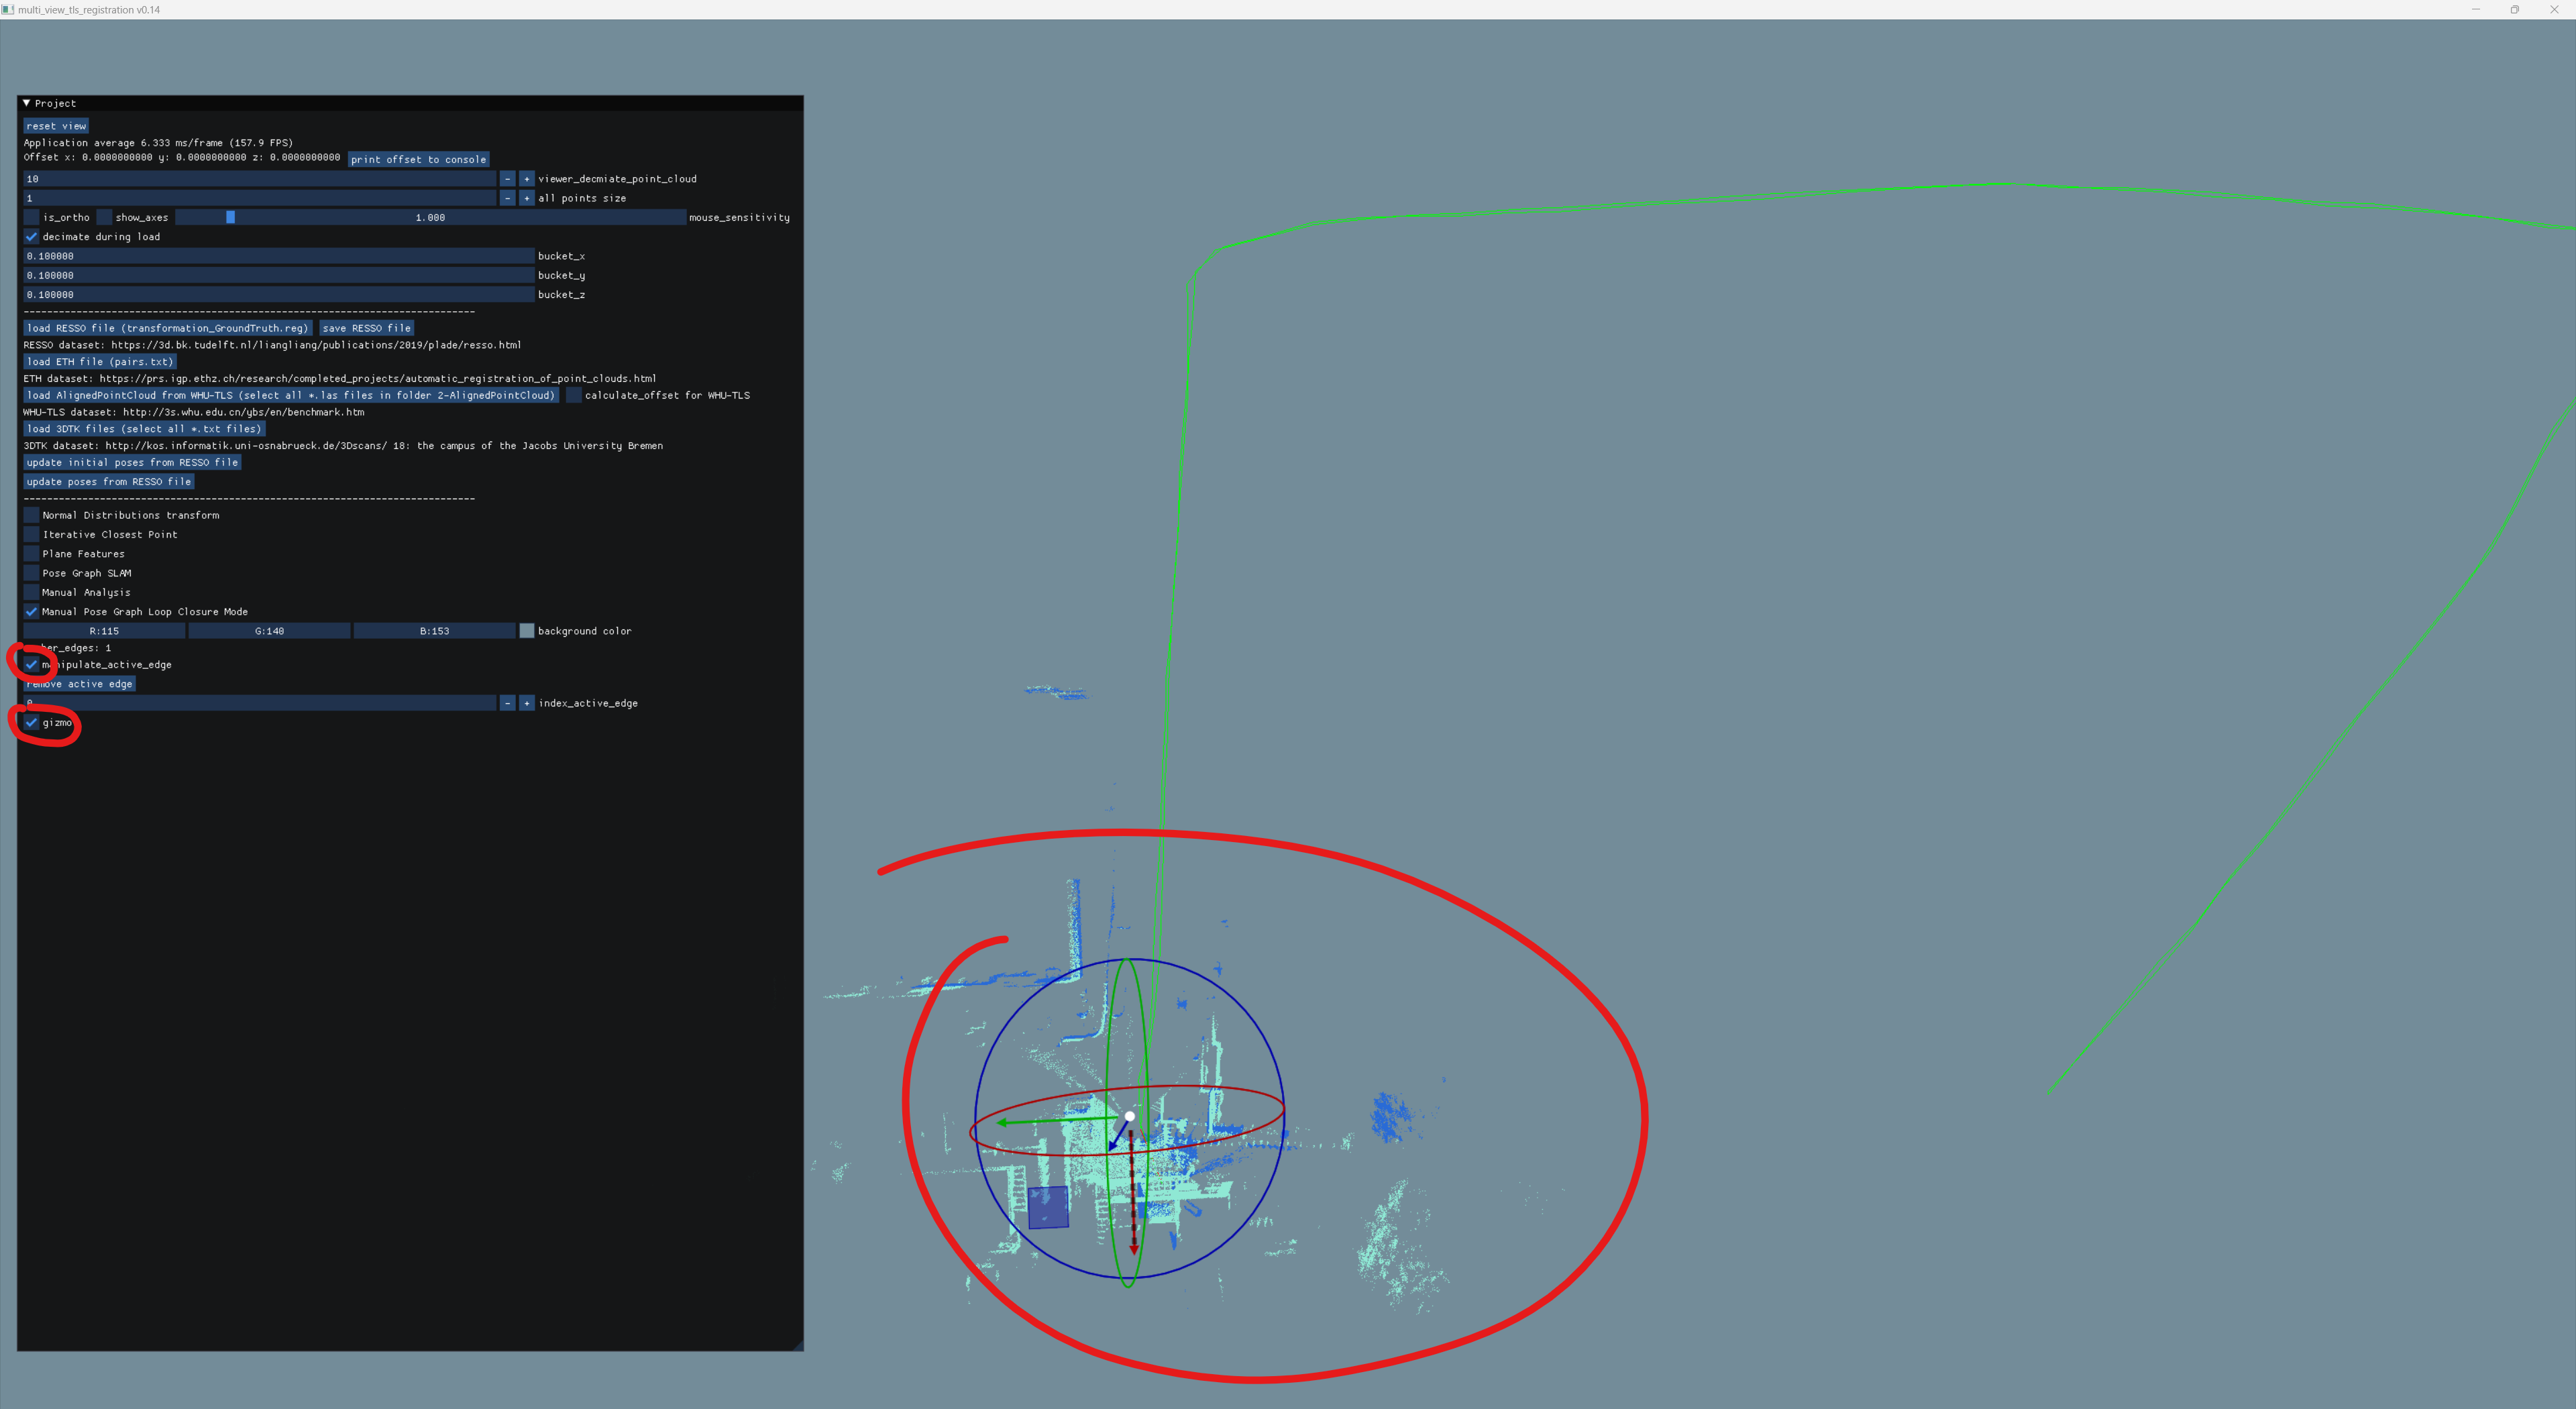
\includegraphics[width=\textwidth]{15.png}
	\caption{Turn on manipulate active edge, turn on gizmo and align scan to scan manually.}
	\label{fig:15}
\end{figure}

\begin{figure}
	\centering
	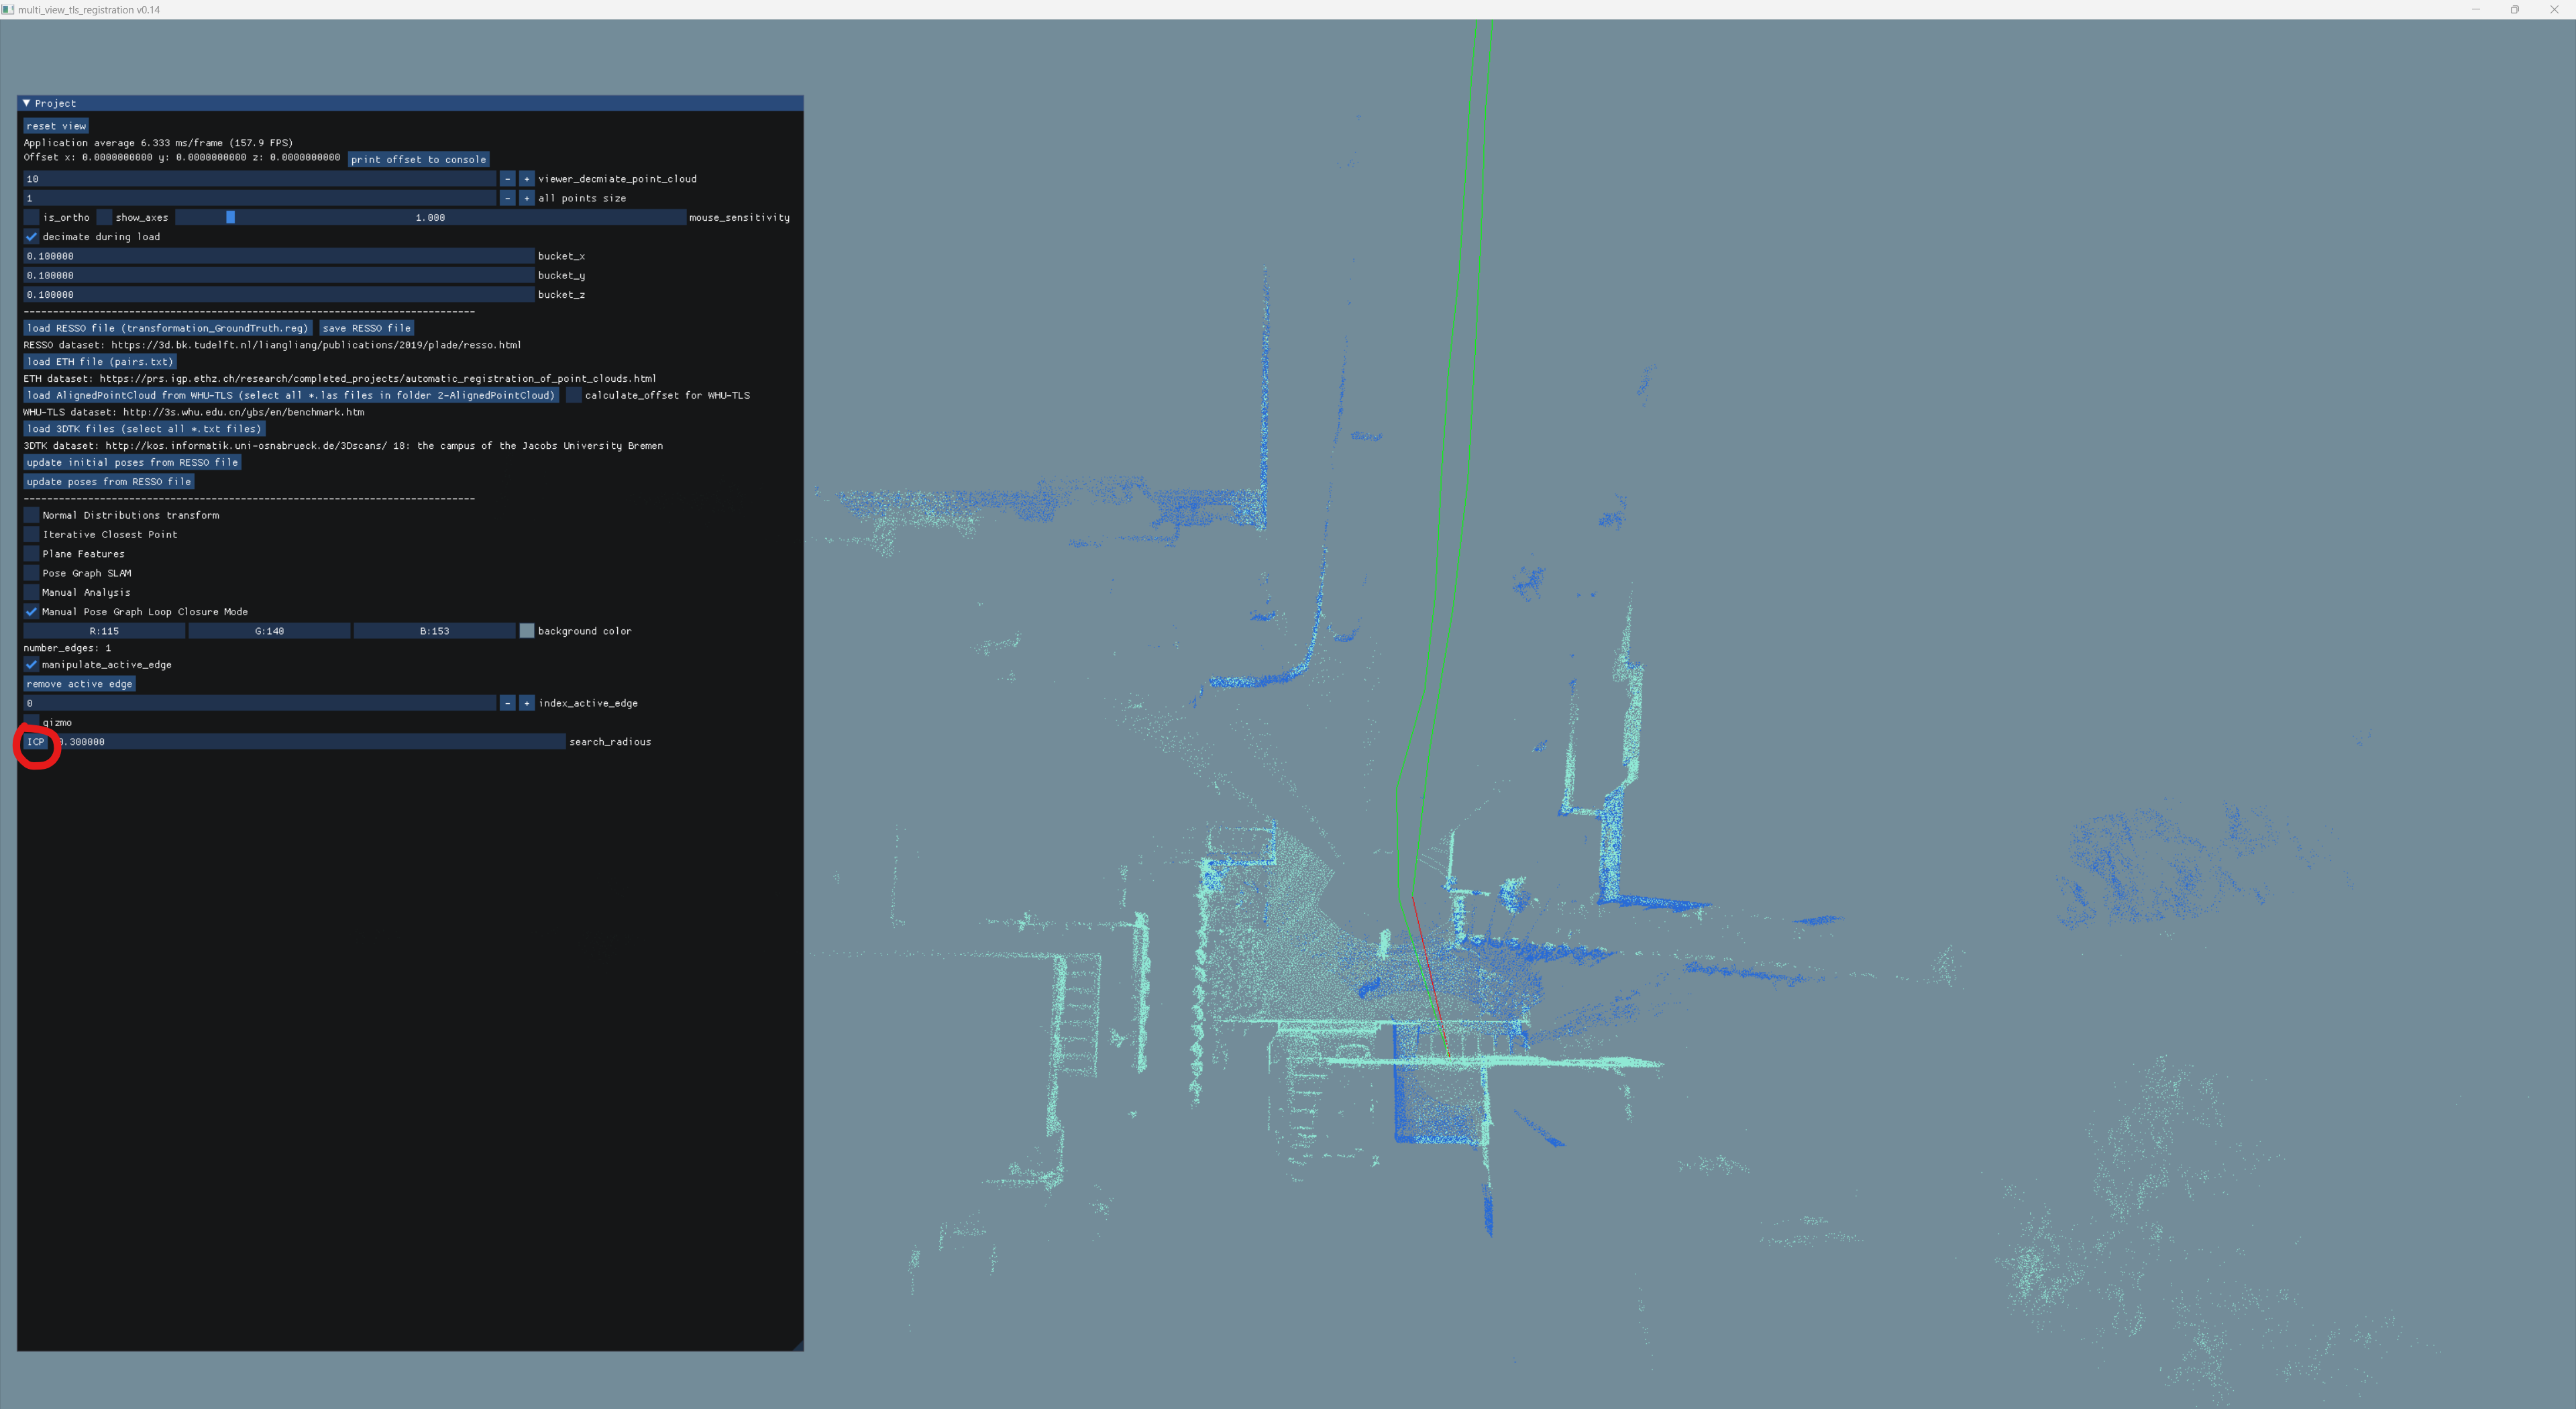
\includegraphics[width=\textwidth]{16.png}
	\caption{Once You are not capable align more accurate, then turn off gizmo and repetitively use ICP until scans align to the level at which nothing can change anymore.}
	\label{fig:16}
\end{figure}

\begin{figure}
	\centering
	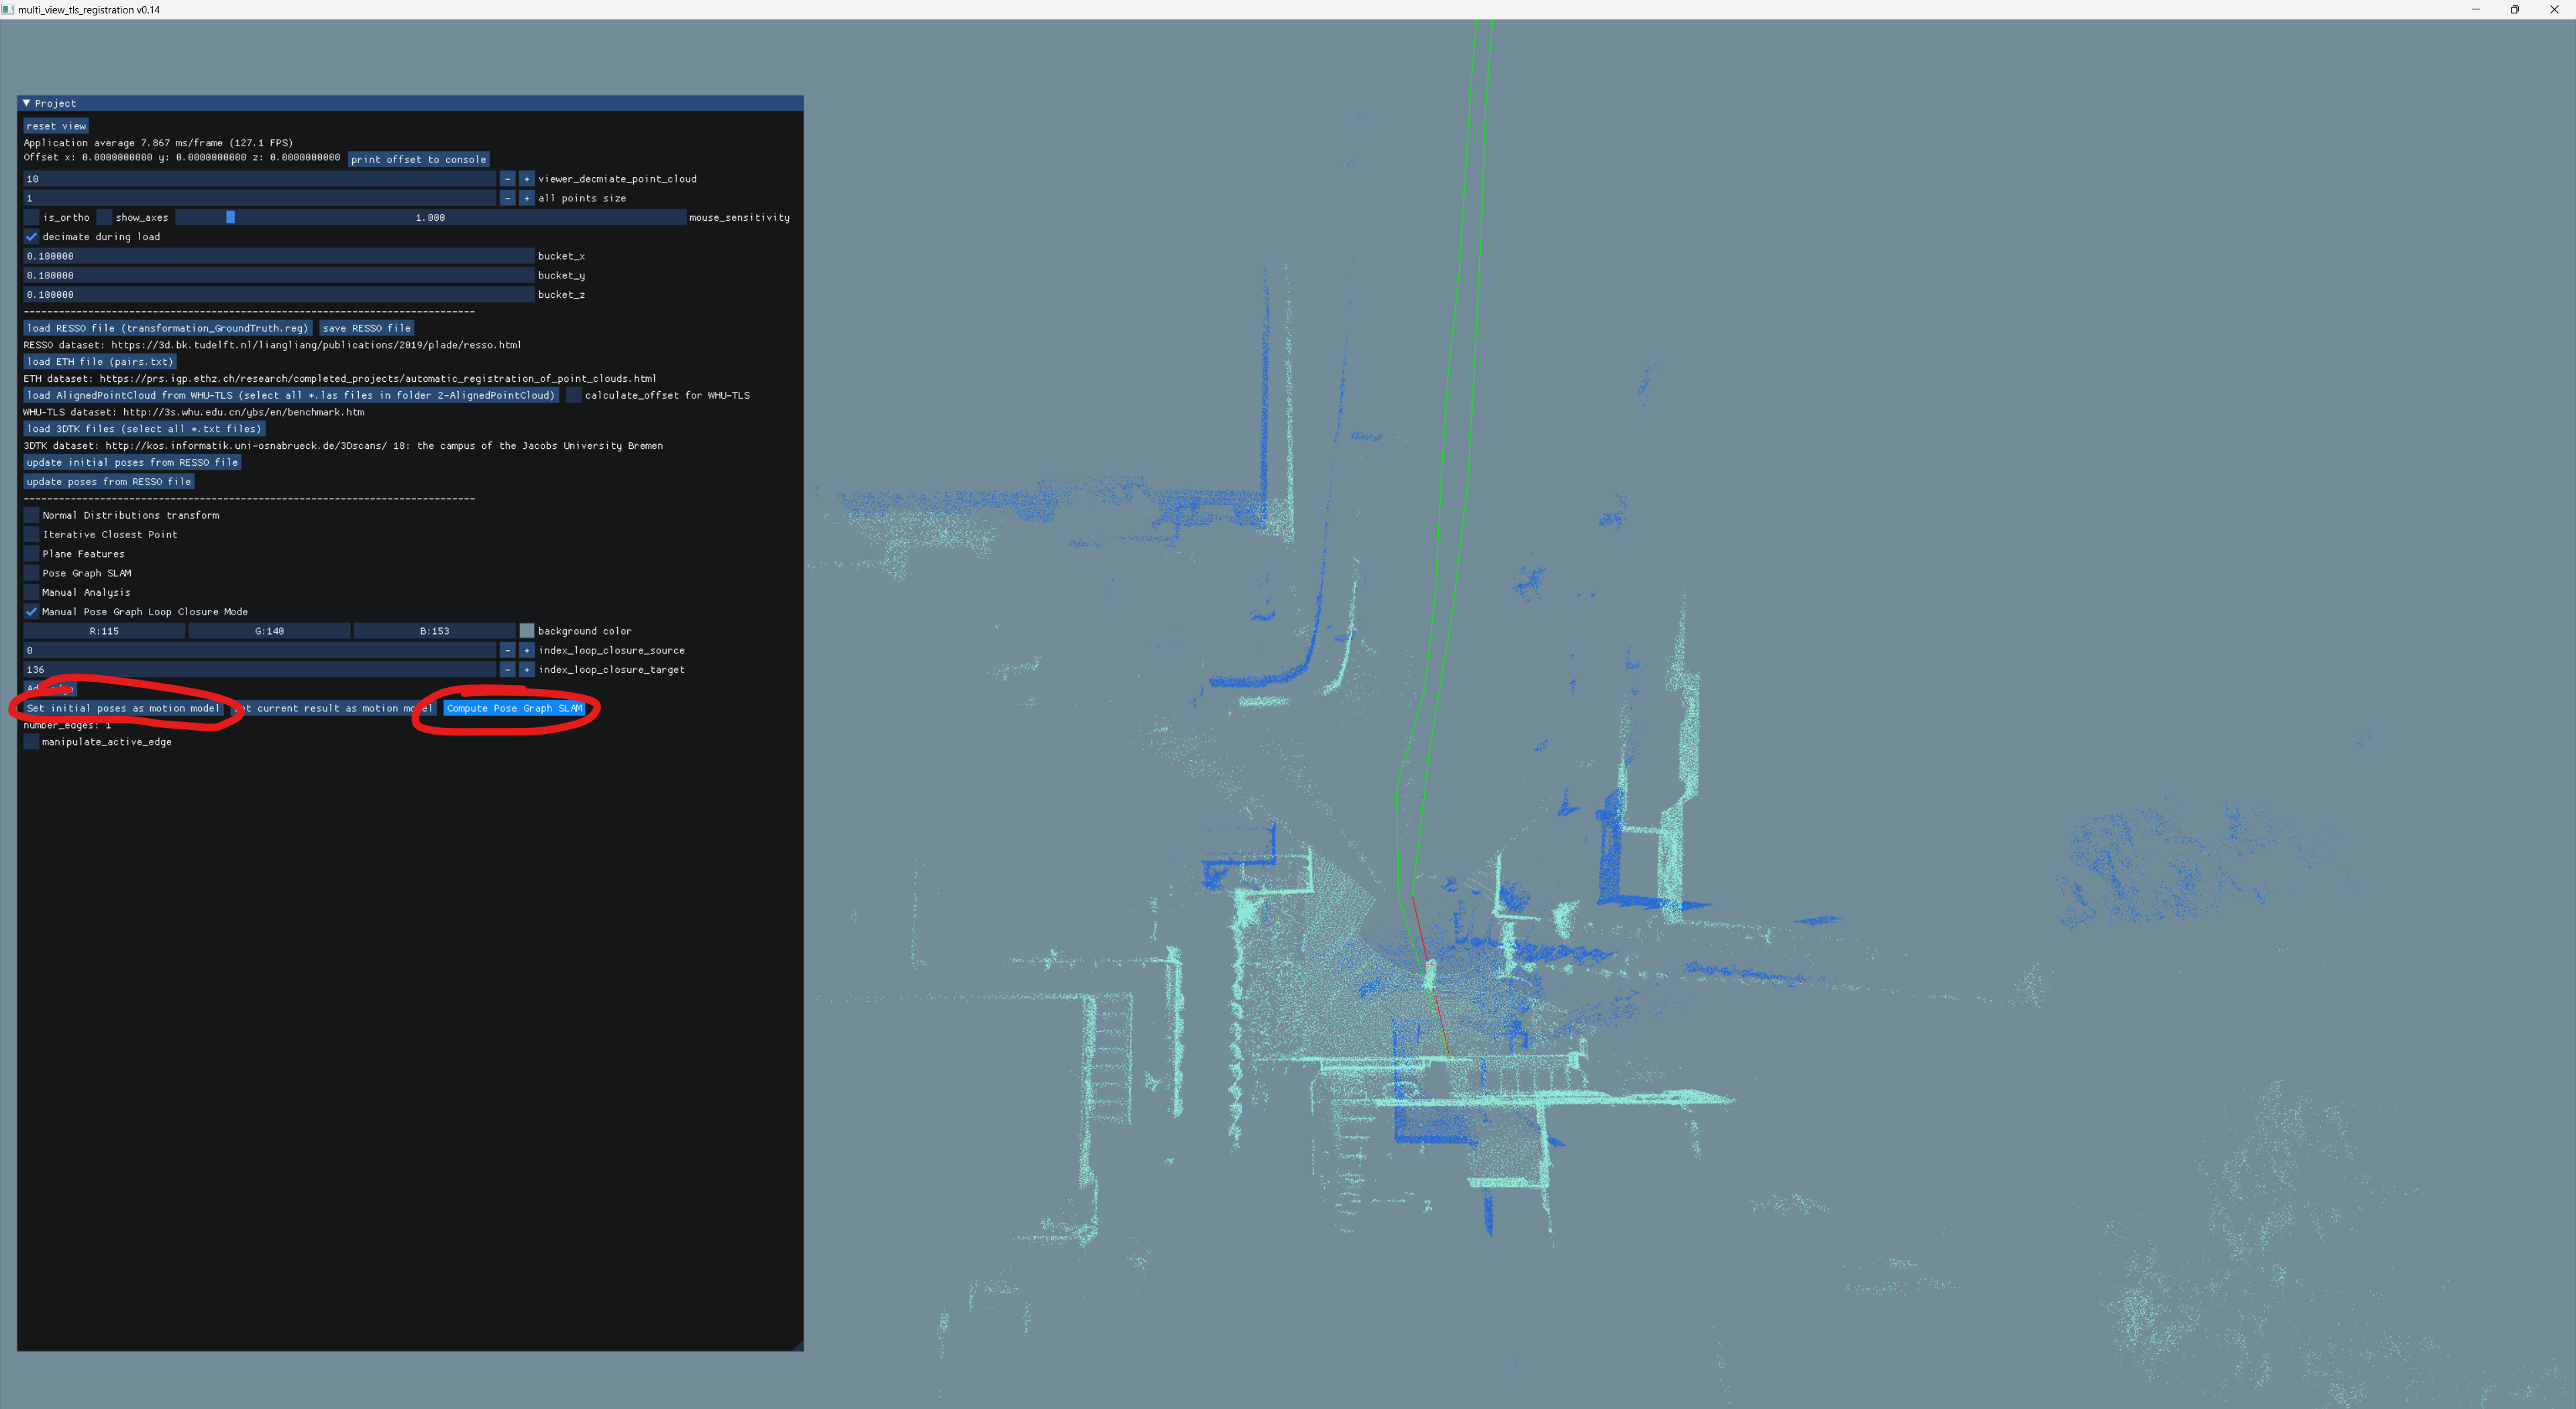
\includegraphics[width=\textwidth]{17.png}
	\caption{Turn off manipulate active edge, click "set initial poses as motion model", then click "compute pose graph SLAM".}
	\label{fig:17}
\end{figure}

\begin{figure}
	\centering
	\includegraphics[width=\textwidth]{18.png}
	\caption{Turn off Manual Pose Graph Loop Closure Mod and inspect if everything is ok, if not,  repeat steps from figures 3.3-3.6 (choose another pair of scans, refine them and compute the pose graph SLAM).}
	\label{fig:18}
\end{figure}

\begin{figure}
	\centering
	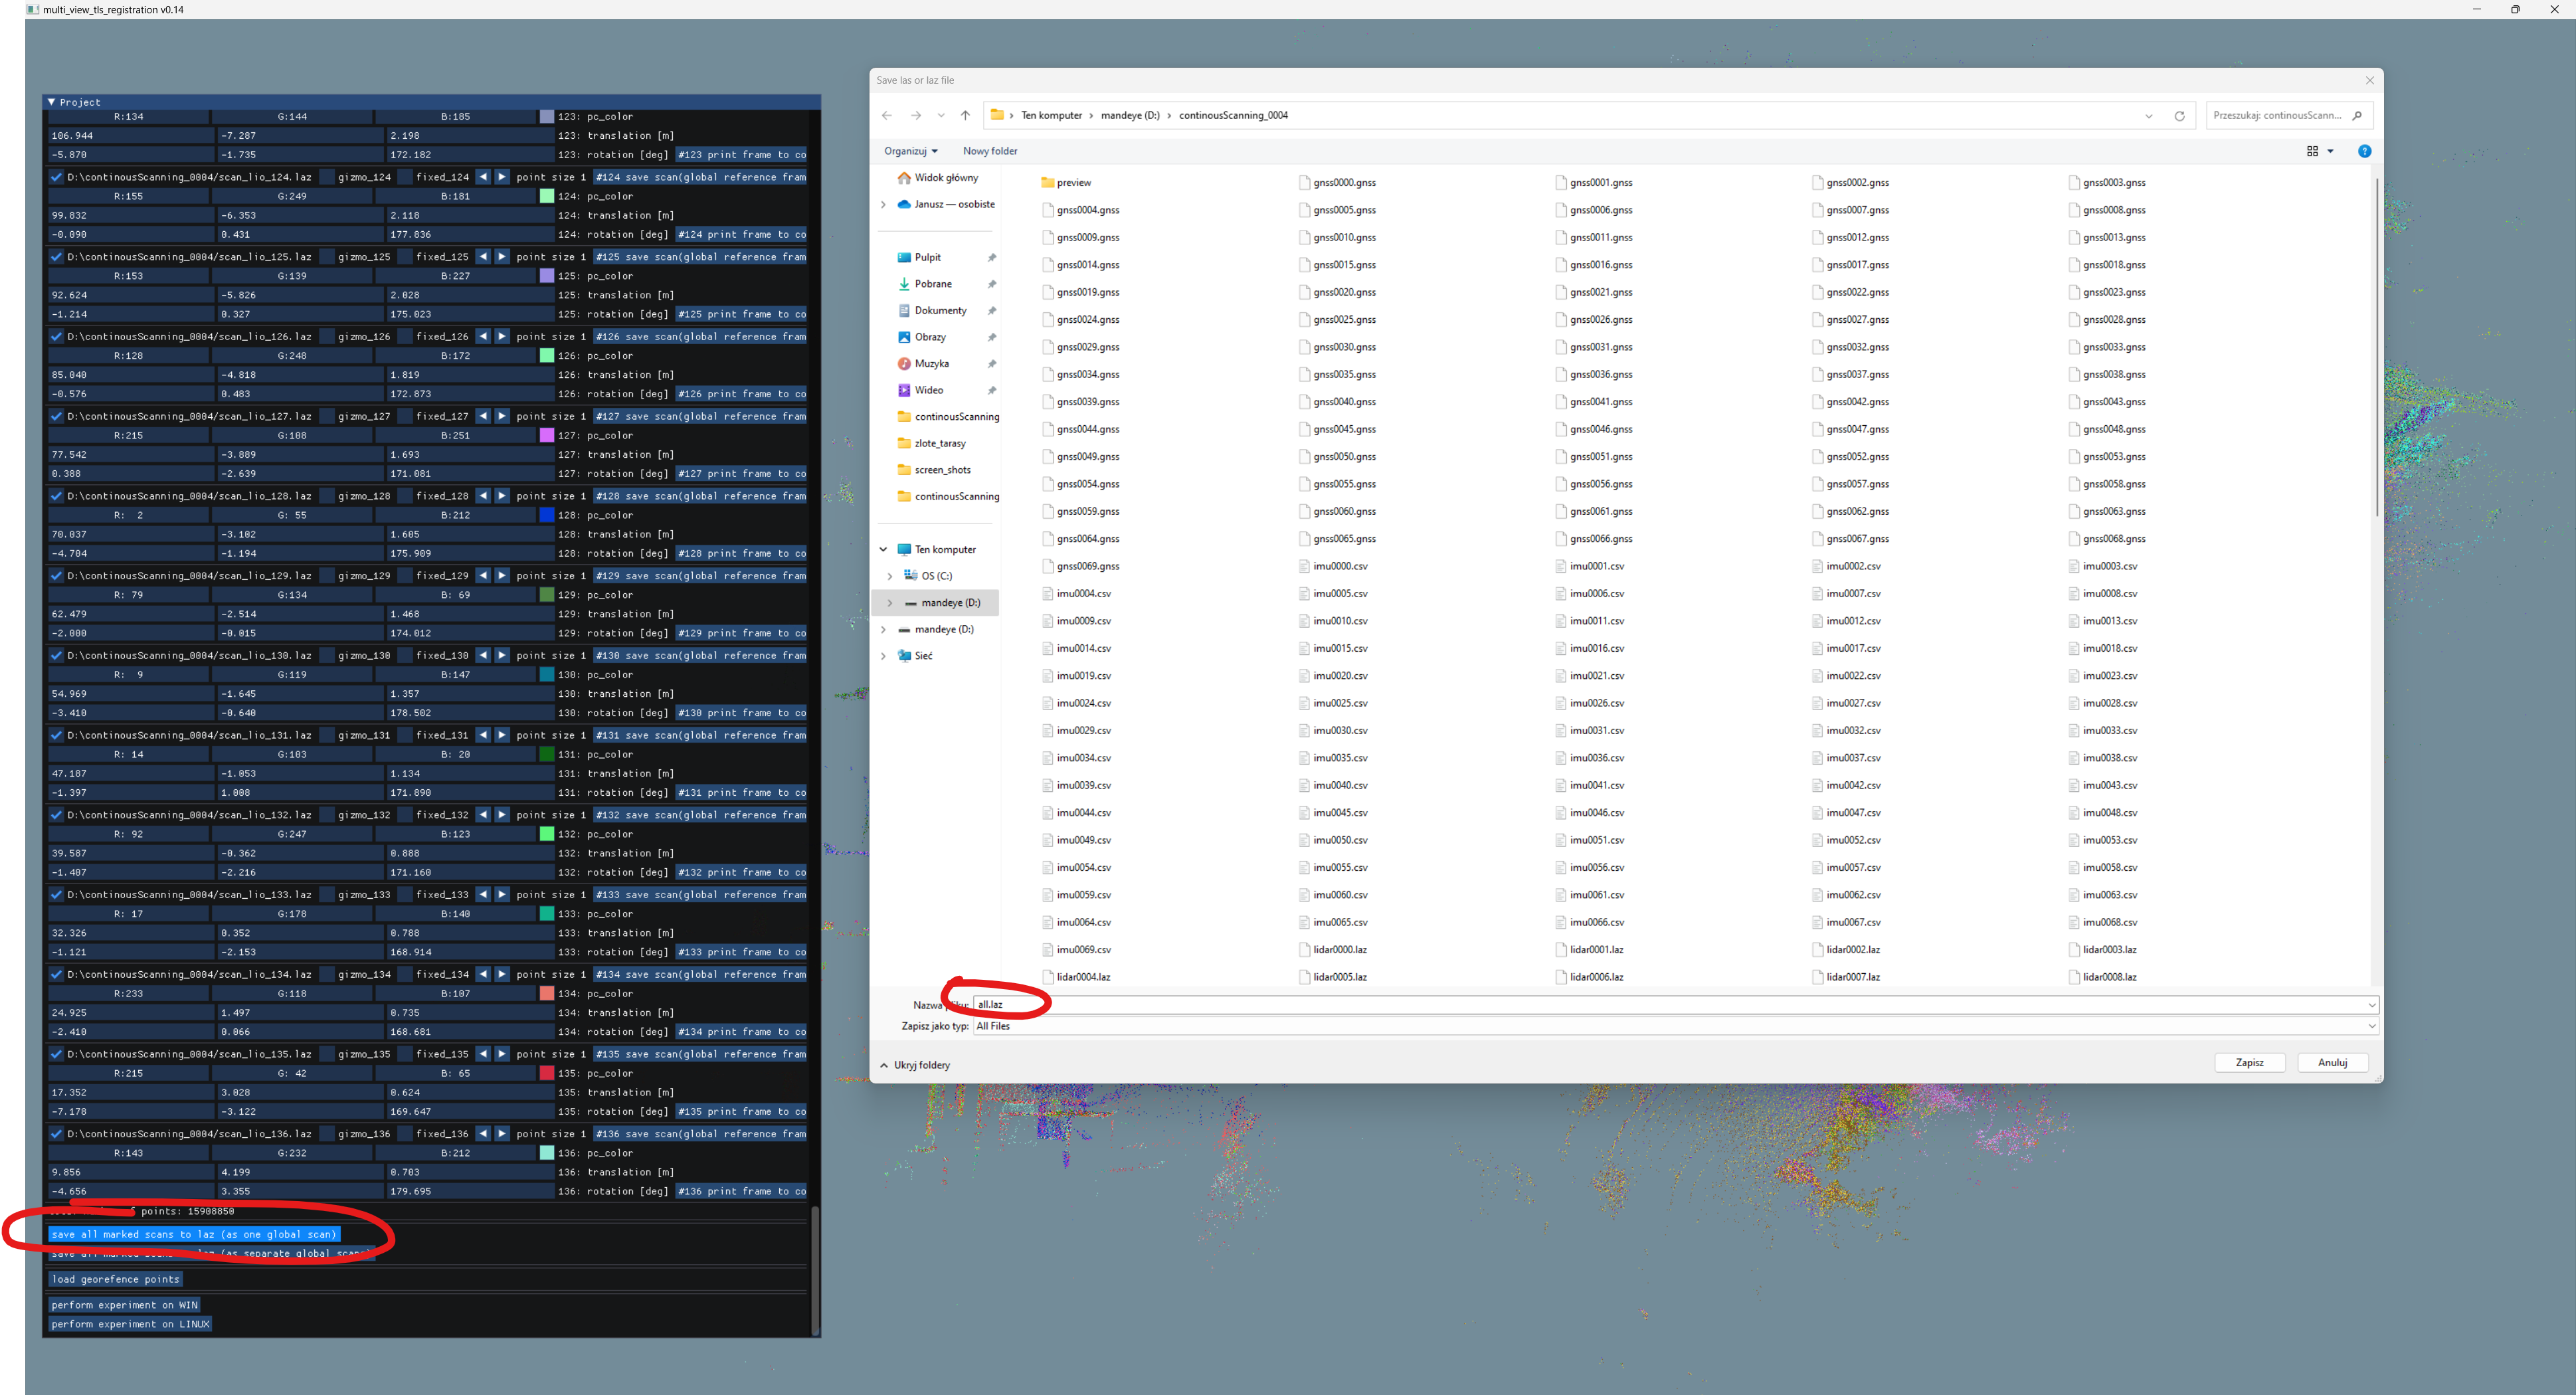
\includegraphics[width=\textwidth]{19.png}
	\caption{Once the job is done export data to *.laz. This is Your map that can be loaded by e.g. \href{https://www.cloudcompare.org/}{CloudCompare}.}
	\label{fig:19}
\end{figure}